% ========================================
%	Header einbinden
% ========================================

\documentclass[bibtotoc,titlepage]{scrartcl}

% Deutsche Spracheinstellungen
\usepackage[ngerman,german]{babel, varioref}
\usepackage[T1]{fontenc}
\usepackage[utf8]{inputenc}

%\usepackage{marvosym}

\usepackage{amsfonts}
\usepackage{amssymb}
\usepackage{amsmath}
\usepackage{amscd}
\usepackage{amstext}
\usepackage{float}
\usepackage{caption}
\usepackage{wrapfig}
\usepackage{setspace}
\usepackage{threeparttable}
\usepackage{footnote}

\newfloat{formel}{htbp}{for}
\floatname{formel}{Formel}


\usepackage{longtable}

%\usepackage{bibgerm}

\usepackage{footnpag}

\usepackage{ifthen}                 %%% package for conditionals in TeX
\usepackage[amssymb]{SIunits}
%Fr textumflossene Bilder und Tablellen
%\usepackage{floatflt} - veraltet

%Fr Testzwecke aktivieren, zeigt labels und refs im Text an.
%\usepackage{showkeys}

% Abstand zwischen zwei Abs�zen nach DIN (1,5 Zeilen)
% \setlength{\parskip}{1.5ex plus0.5ex minus0.5ex}

% Einrckung am Anfang eines neuen Absatzes nach DIN (keine)
%\setlength{\parindent}{0pt}

% R�der definieren
% \setlength{\oddsidemargin}{0.3cm}
% \setlength{\textwidth}{15.6cm}

% bessere Bildunterschriften
%\usepackage[center]{caption2}


% Probleml�ungen beim Umgang mit Gleitumgebungen
\usepackage{float}

% Nummeriert bis zur Strukturstufe 3 (also <section>, <subsection> und <subsubsection>)
%\setcounter{secnumdepth}{3}

% Fhrt das Inhaltsverzeichnis bis zur Strukturstufe 3
%\setcounter{tocdepth}{3}

\usepackage{exscale}

\newenvironment{dsm} {\begin{displaymath}} {\end{displaymath}}
\newenvironment{vars} {\begin{center}\scriptsize} {\normalsize \end{center}}


\newcommand {\en} {\varepsilon_0}               % Epsilon-Null aus der Elektrodynamik
\newcommand {\lap} {\; \mathbf{\Delta}}         % Laplace-Operator
\newcommand {\R} { \mathbb{R} }                 % Menge der reellen Zahlen
\newcommand {\e} { \ \mathbf{e} }               % Eulersche Zahl
\renewcommand {\i} { \mathbf{i} }               % komplexe Zahl i
\newcommand {\N} { \mathbb{N} }                 % Menge der nat. Zahlen
\newcommand {\C} { \mathbb{C} }                 % Menge der kompl. Zahlen
\newcommand {\Z} { \mathbb{Z} }                 % Menge der kompl. Zahlen
\newcommand {\limi}[1]{\lim_{#1 \rightarrow \infty}} % Limes unendlich
\newcommand {\sumi}[1]{\sum_{#1=0}^\infty}
\newcommand {\rot} {\; \mathrm{rot} \,}         % Rotation
\newcommand {\grad} {\; \mathrm{grad} \,}       % Gradient
\newcommand {\dive} {\; \mathrm{div} \,}        % Divergenz
\newcommand {\dx} {\; \mathrm{d} }              % Differential d
\newcommand {\cotanh} {\; \mathrm{cotanh} \,}   %Cotangenshyperbolicus
\newcommand {\asinh} {\; \mathrm{areasinh} \,}  %Area-Sinus-Hyp.
\newcommand {\acosh} {\; \mathrm{areacosh} \,}  %Area-Cosinus-H.
\newcommand {\atanh} {\; \mathrm{areatanh} \,}  %Area Tangens-H.
\newcommand {\acoth} {\; \mathrm{areacoth} \,}  % Area-cotangens
\newcommand {\Sp} {\; \mathrm{Sp} \,}
\newcommand {\mbe} {\stackrel{\text{!}}{=}}     %Must Be Equal
\newcommand{\qed} { \hfill $\square$\\}
\renewcommand{\i} {\imath}
\def\captionsngerman{\def\figurename{\textbf{Abb.}}}

%%%%%%%%%%%%%%%%%%%%%%%%%%%%%%%%%%%%%%%%%%%%%%%%%%%%%%%%%%%%%%%%%%%%%%%%%%%%
% SWITCH FOR PDFLATEX or LATEX
%%%%%%%%%%%%%%%%%%%%%%%%%%%%%%%%%%%%%%%%%%%%%%%%%%%%%%%%%%%%%%%%%%%%%%%%%%%%
%%%
\ifx\pdfoutput\undefined %%%%%%%%%%%%%%%%%%%%%%%%%%%%%%%%%%%%%%%%% LATEX %%%
%%%
\usepackage[dvips]{graphicx}       %%% graphics for dvips
\DeclareGraphicsExtensions{.eps,.ps}   %%% standard extension for included graphics
\usepackage[ps2pdf]{thumbpdf}      %%% thumbnails for ps2pdf
\usepackage[ps2pdf,                %%% hyper-references for ps2pdf
bookmarks=true,%                   %%% generate bookmarks ...
bookmarksnumbered=true,%           %%% ... with numbers
hypertexnames=false,%              %%% needed for correct links to figures !!!
breaklinks=true,%                  %%% breaks lines, but links are very small
linkbordercolor={0 0 1},%          %%% blue frames around links
pdfborder={0 0 112.0}]{hyperref}%  %%% border-width of frames
%                                      will be multiplied with 0.009 by ps2pdf
%
\hypersetup{ pdfauthor   = {Hannes Franke; Julius Tilly},
pdftitle    = {V301 Innenwiderstand und Leistungsanpassung}, pdfsubject  = {Protokoll FP}, pdfkeywords = {V301, Innenwiderstand, Leistungsanpassung},
pdfcreator  = {LaTeX with hyperref package}, pdfproducer = {dvips
+ ps2pdf} }
%%%
\else %%%%%%%%%%%%%%%%%%%%%%%%%%%%%%%%%%%%%%%%%%%%%%%%%%%%%%%%%% PDFLATEX %%%
%%%
\usepackage[pdftex]{graphicx}      %%% graphics for pdfLaTeX
\DeclareGraphicsExtensions{.pdf}   %%% standard extension for included graphics
\usepackage[pdftex]{thumbpdf}      %%% thumbnails for pdflatex
\usepackage[pdftex,                %%% hyper-references for pdflatex
bookmarks=true,%                   %%% generate bookmarks ...
bookmarksnumbered=true,%           %%% ... with numbers
hypertexnames=false,%              %%% needed for correct links to figures !!!
breaklinks=true,%                  %%% break links if exceeding a single line
linkbordercolor={0 0 1},
linktocpage]{hyperref} %%% blue frames around links
%                                  %%% pdfborder={0 0 1} is the default
\hypersetup{
pdftitle    = {V301 Innenwiderstand und Leistungsanpassung}, 
pdfsubject  = {Protokoll AP}, 
pdfkeywords = {V301, Innenwiderstand, Leistungsanpassung},
pdfsubject  = {Protokoll AP},
pdfkeywords = {V301, Innenwiderstand, Leistungsanpassung}}
%                                  %%% pdfcreator, pdfproducer,
%                                      and CreationDate are automatically set
%                                      by pdflatex !!!
\pdfadjustspacing=1                %%% force LaTeX-like character spacing
\usepackage{epstopdf}
%
\fi %%%%%%%%%%%%%%%%%%%%%%%%%%%%%%%%%%%%%%%%%%%%%%%%%%% END OF CONDITION %%%
%%%%%%%%%%%%%%%%%%%%%%%%%%%%%%%%%%%%%%%%%%%%%%%%%%%%%%%%%%%%%%%%%%%%%%%%%%%%
% seitliche Tabellen und Abbildungen
%\usepackage{rotating}
\usepackage{ae}
\usepackage{
  array,
  booktabs,
  dcolumn
}
\makeatletter 
  \renewenvironment{figure}[1][] {% 
    \ifthenelse{\equal{#1}{}}{% 
      \@float{figure} 
    }{% 
      \@float{figure}[#1]% 
    }% 
    \centering 
  }{% 
    \end@float 
  } 
  \makeatother 


  \makeatletter 
  \renewenvironment{table}[1][] {% 
    \ifthenelse{\equal{#1}{}}{% 
      \@float{table} 
    }{% 
      \@float{table}[#1]% 
    }% 
    \centering 
  }{% 
    \end@float 
  } 
  \makeatother 
%\usepackage{listings}
%\lstloadlanguages{[Visual]Basic}
%\allowdisplaybreaks[1]
%\usepackage{hycap}
%\usepackage{fancyunits}

% ========================================
%	Angaben für das Titelblatt
% ========================================

\title{Versuch 48 - Dipolrelaxation in Ionenkristallen\\				% Titel des Versuchs 
\large TU Dortmund, Fakultät Physik\\ 
\normalsize Fortgeschrittenen-Praktikum}

\author{Jan Adam\\			% Name Praktikumspartner A
{\small \href{jan.adam@tu-dortmund.de}{jan.adam@tu-dortmund.de}}	% Erzeugt interaktiven einen Link
\and						% um einen weiteren Author hinzuzfügen
Dimitrios Skodras\\					% Name Praktikumspartner B
{\small \href{dimitrios.skodras@tu-dortmund.de}{dimitrios.skodras@tu-dortmund.de}}		% Erzeugt interaktiven einen Link
}
\date{16. April 2014}				% Das Datum der Versuchsdurchführung

% ========================================
%	Das Dokument beginnt
% ========================================

\begin{document}

% ========================================
%	Titelblatt erzeugen
% ========================================

\maketitle					% Jetzt wird die Titelseite erzeugt
\thispagestyle{empty} 				% Weder Kopfzeile noch Fußzeile

% ========================================
%	Der Vorspann
% ========================================

%\newpage					% Wenn Verzeichnisse auf einer neuen Seite beginnen sollen
%\pagestyle{empty}				% Weder Kopf- noch Fußzeile für Verzeichnisse

\tableofcontents

%\newpage					% eine neue Seite
%\thispagestyle{empty}				% Weder Kopf- noch Fußzeile für Verzeichnisse
%\listoffigures					% Abbildungsverzeichnis

%\newpage					% eine neue Seite
%\thispagestyle{empty}				% Weder Kopf- noch Fußzeile für Verzeichnisse
%\listoftables					% Tabellenverzeichnis
\newpage					% eine neue Seite


% ========================================
%	Kapitel
% ========================================

%\section{Einleitung}				% Bei Bedarf

\section{Theorie}
\setcounter{page}{1}
\subsection{Ionengitter}
Ein einwertiger Ionenkristall (CsJ) erfährt einen Einbau eines zweiwertigen Kations (Sr$^{++}$), wodurch ein permanenter Dipol entsteht. Denn aufgrund
der Ladungserhaltung entsteht mit dem zweiwertigen Kation eine Leerstelle, die gemeinsam entsprechend Abbildung \ref{pic_dipGitt} den Dipol bilden.
\begin{figure}[H]
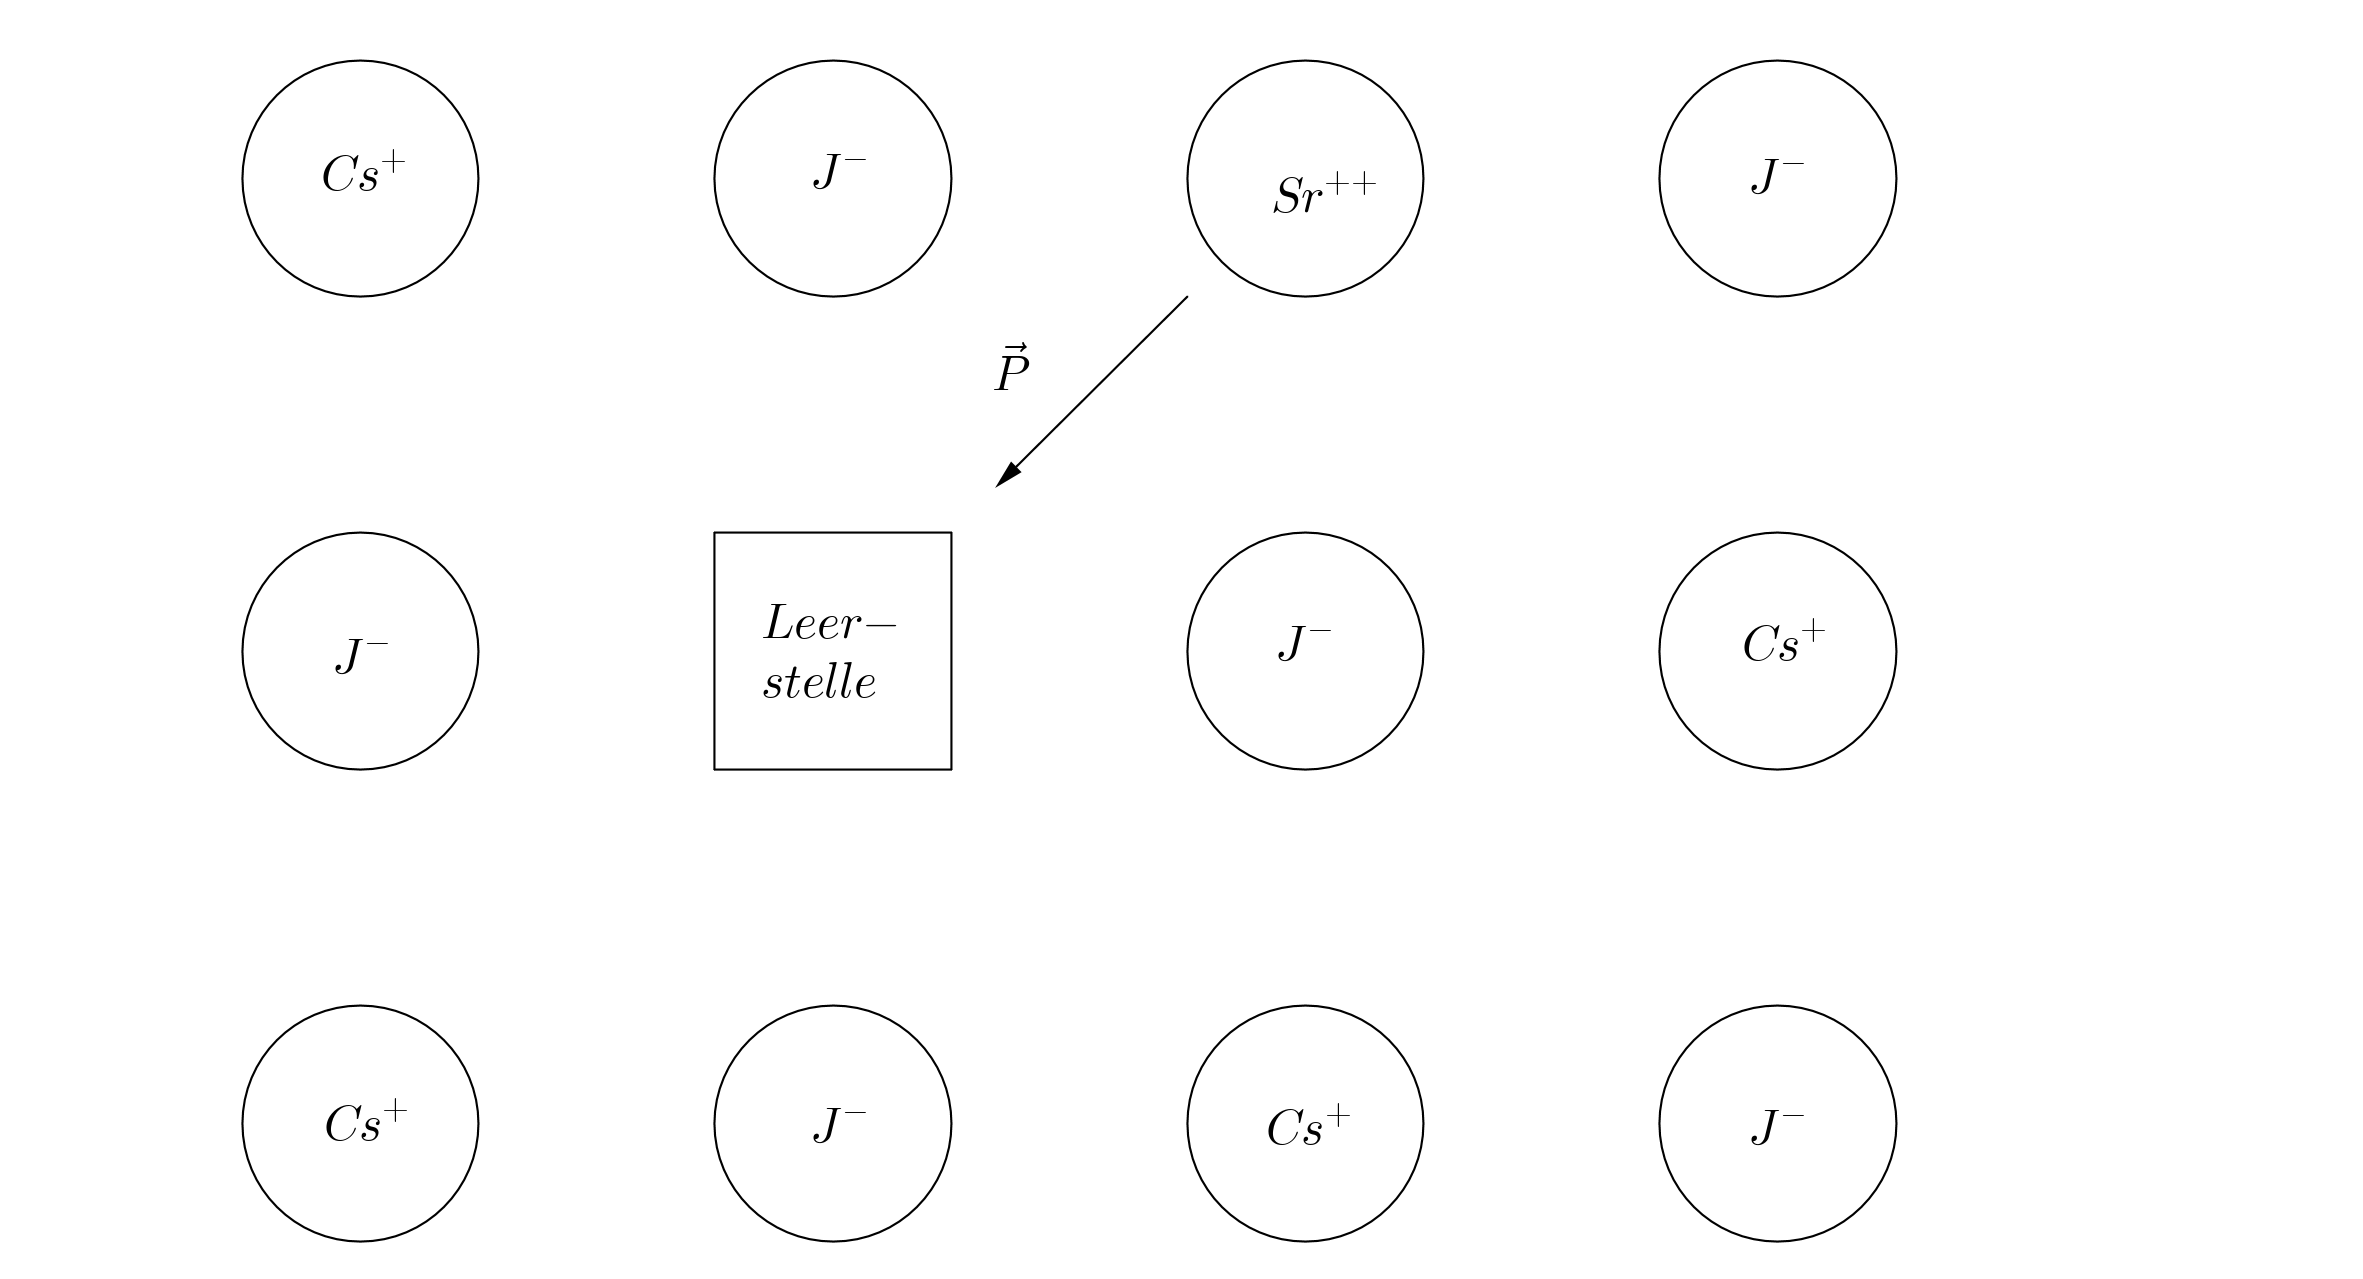
\includegraphics[width=\textwidth]{../pics/dipGitt.png}
\caption{Entstehung eines Dipols im Ionengitter}
\label{pic_dipGitt}
\end{figure}
Wegen der diskreten Gitterpunkte sind nur diskrete Dipolausrichtung möglich, wobei unterhalb von 500 $^\circ$C sich ausschließlich die Leerstellen bewegen.
Die Potentialschwelle die zu dieser Leerstellendiffusion die durch den periodischen Verlauf des Gitterpotentials festgelegt ist, muss überwunden werden.
Damit ist eine Aktivierungsenergie $W$ verbunden. Der Anteil der Dipole, die diese Energie mittels der thermischen Bewegung aufbringt ist
verteilt nach der Boltzmann-Statistik $\exp(W/k_B\,T)$, mit $k_B$ als Boltzmann-Konstante. Die mittlere Zeit einer Dipolumorientierung wird Relaxationszeit
$\tau$ genannt, die direkt proportional zur Boltzmann-Statistik sein muss
\begin{align}
 \tau(T) = \tau_0 \exp\left(\frac{W}{k_B\, T}\right),
\end{align}
mit $\tau_0$ als charakteristische Relaxationszeit, die bei unendlicher Temperatur bestehen würde. Im Versuch sollen die Aktivierungsenergie und die
charakteristische Relaxationszeit ermittelt werden.

\subsection{Messverfahren}
Die untersuchte mit Strontium dotierte Kaliumbromid-Probe ist kreisförmig und etwa 3-5 mm dick. Sie dient als Dielektrikum eines Plattenkondensators,
an den eine Gleichspannung angeschlossen wird, sodass innerhalb der Probe ein elektrisches Feld $E$ wirkt. Die statistisch ausgerichteten 
Dipole in der Probe richten sich entsprechend der Feldrichtung aus. Die Ausrichtung wird jedoch wird jedoch durch die thermische Bewegung der 
Gitterbausteine gestört, sodass nur ein Bruchteil $y$ der Dipole in Feldrichtung zeigt. Dieser Anteil wird durch die Langevin-Funktion $L(x)$
beschrieben
\begin{align}
 y = L(x) = \cot(x) - \frac{1}{x} \hspace{1cm}\text{mit }x=\frac{pE}{k_B T},
\end{align}
die für den Fall $pE\ll k_B T$ wird zu 
\begin{align}
 y = \frac{pE}{3k_B T}.
\end{align}
Um tatsächlich diesen Bruchteil zu erhalten, muss das Feld lange gegenüber der Relaxationszeit eingeschaltet sein. Bei eingeschaltetem E-Feld wird
die Probe mit flüssigem Stickstoff schnell auf eine Temperatur $T_0$ gebracht. Wegen des exponentiellen Zusammenhangs, ist es möglich, diesen
Polarisationszustand konstant zu halten. Nach Abschalten des Felds, wird der Kondensator kurzgeschlossen, was den Ladungsteil bei tiefen Temperaturen
in Form von Elektronen verschwinden lässt. Mit konstanter Heizrate $b=\dx T/\dx t = const$ wird die Probe erhitzt, was dazu führt, dass die Dipole
sich wieder statistisch ausrichten werden. Dieser Vorgang wird Dipolrelaxation genannt und bringt einen Depolarisationsstrom mit sich, der mit einem
empfindlichen Strommessgerät gemessen werden kann. Zu Beginn steigt der Strom entsprechend Abbildung \ref{pic_i(T)} mit der Temperatur steil an, da $\tau$ schnell abnimmt, woraufhin er
ein Maximum erreicht und wieder abnimmt, da nicht relaxierte Dipole weniger werden. Die Depolarisationsstromdichte $j(T)$ setzt sich zusammen aus dem
Bruchteil $y$, der bei Polarisationstemperatur $T_p$ orientierten Dipole, dem Dipolmoment $p$ und der Zahl der pro Zeiteinheit relaxierenden Dipole
$\dx N/\dx t$
\begin{align}
 j(T) = y(T_p)\, p\, \frac{\dx N}{\dx t}.
\end{align}
\begin{figure}[H]
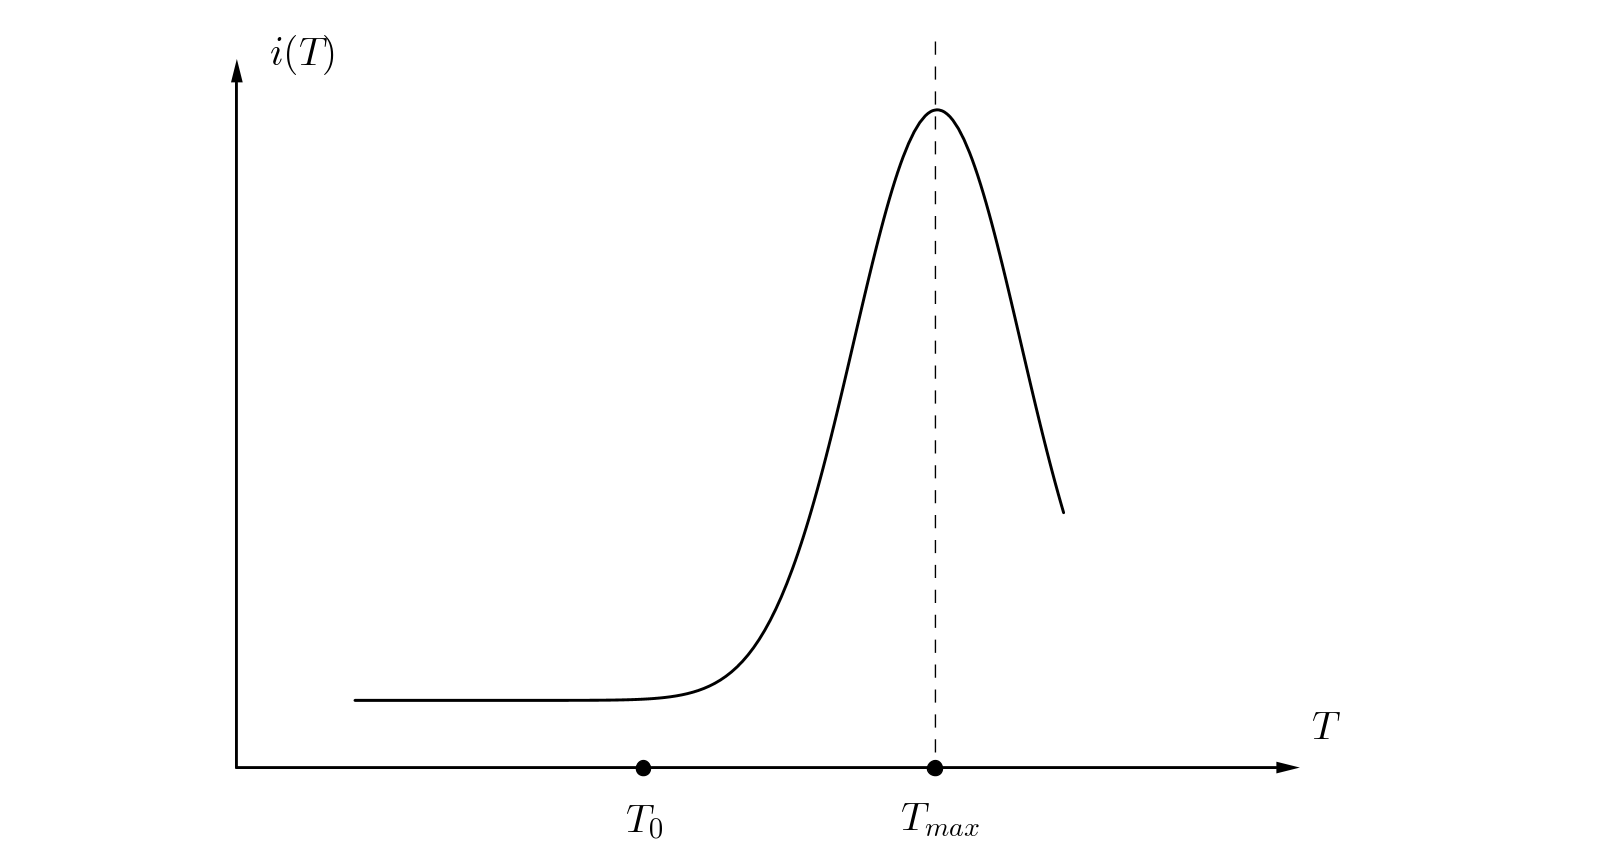
\includegraphics[width=\textwidth]{../pics/i(T).png}
\caption{Depolarisationsstromdichte}
\label{pic_i(T)}
\end{figure}


\section{Durchführung}

\section{Auswertung}

\parskip 340pt
\Large{Literatur}\\\\

% ========================================
%	Literaturverzeichnis
% ========================================

%\bibliographystyle{plainnat}			% Bibliographie-Style auswählen
%\bibliography{BIBDATEI}			% Literaturverzeichnis

% ========================================
%	Das Dokument endent
% ========================================

\end{document}
